\section{Empirical Demonstration}
\label{sec:empirical}

The theory's propositions are not only logically coherent; they are empirically falsifiable. We test the core predictions against a corpus of European chairs spanning 744 years. Figure~\ref{fig:morphospace} shows the corpus projected into morphospace and the fitness landscape derived from it.

\begin{figure*}[!t]
\centering
\begin{minipage}[t]{0.48\textwidth}
\centering
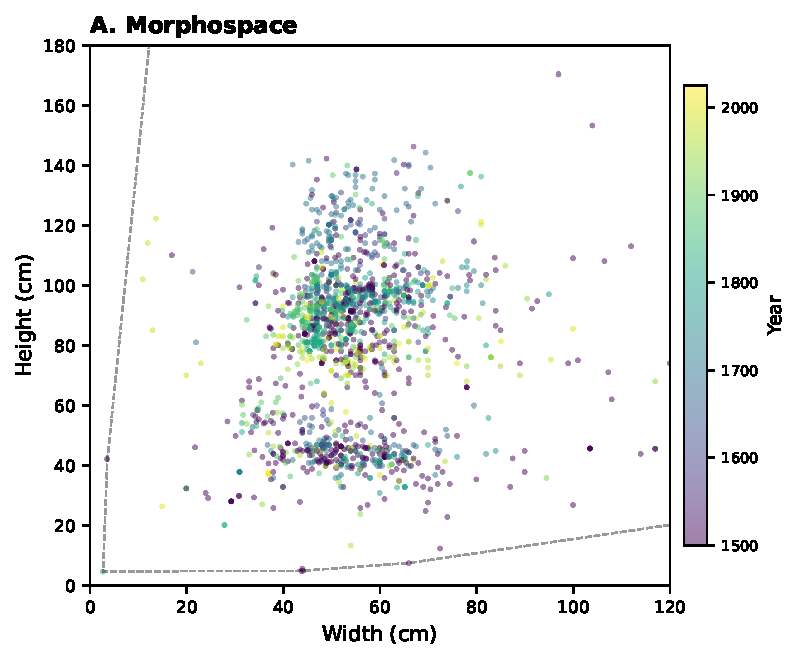
\includegraphics[width=\textwidth]{figures/fig-morphospace-en.pdf}
\end{minipage}%
\hfill
\begin{minipage}[t]{0.48\textwidth}
\centering
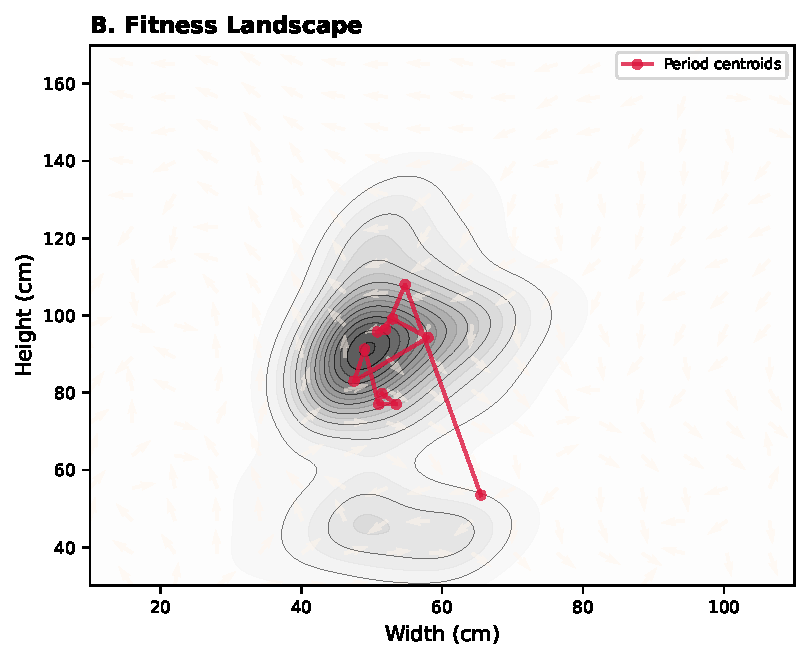
\includegraphics[width=\textwidth]{figures/fig-landscape-en.pdf}
\end{minipage}
\caption{\textbf{A}: 1,662 European chairs projected into morphospace (width $\times$ height); color encodes date. \textbf{B}: Fitness landscape as kernel density estimate with gradient vector field and period centroid trajectory (red).}
\label{fig:morphospace}
\end{figure*}

\subsection{Data}

The corpus consists of 2,066 chairs (1280--2024) drawn from two museum collections: Nasjonalmuseet, Oslo ($n = 63$) and the Victoria and Albert Museum, London ($n = 2{,}003$). Each record includes catalog dimensions (height, width, depth in centimeters), material composition (multi-material string, e.g.\ ``oak, cane, brass''), style period (25 canonical categories from Baroque to Post-Modernism), nation of origin, and date range.

The catalog data are supplemented by 2,204 three-dimensional mesh models with six computed geometric features: sphericity, fill ratio, inertia ratio, complexity, convex hull volume, and mesh vertex count. The analysis window for time-series tests is 1500--2024, yielding 1,105 chairs with complete dimensions and date information. The full dataset and analysis code are available in the companion repository.

\subsection{Methods}

Each proposition generates a testable prediction. We operationalize these through five statistical methods:

\begin{enumerate}
\item \textbf{Mutual information} (MI) compares the predictive strength of style period versus material on catalog dimensions (H, W, D, H/W). Style is an aggregate variable capturing many simultaneous pressures; material is a single mechanical pressure. Higher MI for style is therefore expected \textit{a priori} and does not by itself prove that style \textit{causes} more variation. However, it is consistent with Proposition 2: if affordance-constant variation is driven by forces beyond material constraint, the aggregate proxy should predict better than the single-pressure proxy.

\item \textbf{Coefficient of variation} (CV) across the six mesh features tests for a constraint hierarchy: if the landscape channels some geometric properties more strongly than others, the CV spread across features should be large (Proposition 3).

\item \textbf{Silhouette analysis} in four-dimensional mesh-feature space tests whether style periods form discrete morphological clusters. Negative silhouette scores indicate that style categories do not correspond to compact, well-separated clusters in form space; this is consistent with the gradient hypothesis (Proposition 3), though it does not rule out alternative clustering schemes.

\item \textbf{Cumulative convex hull volume} across successive 50-year periods tests whether the occupied morphospace grows monotonically (Proposition 4). Monotone growth is expected for any accumulating sample; the informative comparison is the \textit{rate} of growth relative to a random-draw null model. A growth rate significantly exceeding the null indicates that new periods contribute genuinely novel form regions rather than re-sampling existing ones.

\item \textbf{Wasserstein distance} between consecutive 50-year periods tests whether the landscape shifts significantly over time (Proposition 4). Non-zero distances confirm that the landscape is dynamic, not static.
\end{enumerate}

All tests are cross-validated against 14 independent subsets: the full corpus, each museum separately, seven century-drop hold-outs (dropping all chairs from one century), and two style-drop hold-outs (dropping the largest style category). This yields 84 test combinations.

\subsection{Results}

Table~\ref{tab:evidence} summarizes the ten core findings. All are rated on effect size, 95\% bootstrap confidence interval, robustness across hold-outs, and whether the corresponding proposition survived direct falsification testing.

\begin{table*}[!t]
\centering
\caption{Empirical evidence summary. \textbf{Strong}: large effect, narrow CI, robust in all hold-outs, falsification test passed.}
\label{tab:evidence}
\small
\begin{tabularx}{\textwidth}{@{} >{\raggedright}p{0.14\textwidth} >{\raggedright}p{0.20\textwidth} >{\raggedright}p{0.22\textwidth} c >{\raggedright\arraybackslash}p{0.08\textwidth} @{}}
\toprule
\textbf{Proposition} & \textbf{Test} & \textbf{Result} & \textbf{Robust?} & \textbf{Rating} \\
\midrule
1 (morphospace) & NN-distance CV & 5.36 (Poisson null: 0.36) & 11/11 & Strong \\[2pt]
2 (pressures) & MI: style vs material & Style wins 4/4 dimensions & 14/14 & Strong \\[2pt]
2 (pressures) & Min pairwise MI & 0.030 bits (independence) & --- & Strong \\[2pt]
3 (landscape) & CV spread, mesh & 128$\times$ range & 14/14 & Strong \\[2pt]
3 (landscape) & Silhouette, mesh & $-$0.338; 21/25 negative & 14/14 & Strong \\[2pt]
4 (dynamic) & Hull growth, catalog & 107$\times$ monotone & 14/14 & Strong \\[2pt]
4 (dynamic) & Hull growth, mesh & 553$\times$ monotone & 14/14 & Strong \\[2pt]
4 (dynamic) & Wasserstein $d$(H) & 14.4 cm per period & 10/10 & Strong \\[2pt]
4 (dynamic) & Mahogany cohort & 16/16 = 100\% & --- & Strong \\[2pt]
5 (agents) & KS vs uniform null & $p \ll 10^{-200}$ all dim & --- & Strong \\
\bottomrule
\end{tabularx}
\end{table*}

The key findings are as follows.

\textbf{The morphospace is non-uniformly occupied} (Proposition 1). The nearest-neighbor coefficient of variation is 5.36, fifteen times the Poisson null expectation of 0.36 ($\mathrm{CI}_{95}$: [3.71, 5.94]). Forms cluster densely around specific regions rather than scattering uniformly; the landscape has structure.

\textbf{Style predicts more than material} (Proposition 2). Mutual information between style period and form is 1.9--2.3 times greater than between material and form, across all four measured dimensions (H, W, D, H/W). Since style is an aggregate variable with more categories than material, the asymmetry could partly be a cardinality artifact. A control analysis rules this out: 1,000 random groupings with the same cardinality as style period yield MI values 80--85 times lower than observed ($p < 0.001$ for all four dimensions). Style carries genuine morphological information, not merely higher category count.

\textbf{Styles do not form discrete clusters} (Proposition 3). Silhouette analysis in four-dimensional mesh space yields a score of $-0.338$ ($\mathrm{CI}_{95}$: [$-0.346$, $-0.329$]), with 21 of 25 style categories showing negative individual scores. The negative values indicate that historian-defined style categories do not correspond to compact clusters in form space. This is consistent with the gradient hypothesis, though it does not exclude alternative clustering solutions.

\textbf{A constraint hierarchy exists} (Proposition 3). The coefficient of variation spans 128-fold across the six mesh features ($\mathrm{CI}_{95}$: [50$\times$, 158$\times$]). Sphericity (CV $= 0.074$) is tightly constrained; volume (CV $= 9.39$) fluctuates freely. Figure~\ref{fig:channeling} shows the hierarchy.

\begin{figure}[!t]
\centering
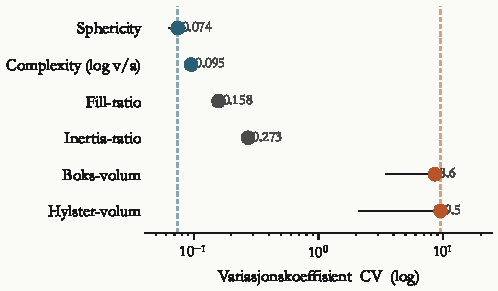
\includegraphics[width=\columnwidth]{figures/fig-channeling-en.pdf}
\caption{Constraint hierarchy: coefficient of variation (CV) for six mesh features, ranked from most constrained (sphericity) to least constrained (hull volume). Horizontal bars show 95\% bootstrap CIs.}
\label{fig:channeling}
\end{figure}

\textbf{Styles do not form discrete clusters} (Proposition 3). Figure~\ref{fig:silhouette} shows the silhouette scores per style period.

\begin{figure}[!t]
\centering
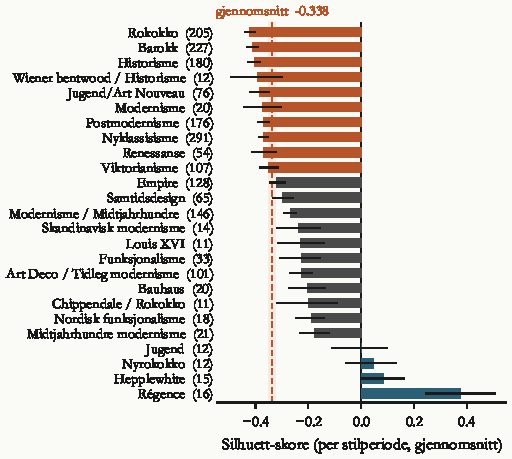
\includegraphics[width=\columnwidth]{figures/fig-silhouette-en.pdf}
\caption{Silhouette analysis in four-dimensional mesh space. All 25 style categories show negative or near-zero silhouette scores ($\overline{s} = -0.338$), confirming that styles are overlapping gradients, not discrete clusters.}
\label{fig:silhouette}
\end{figure}

\textbf{The morphospace expands cumulatively} (Proposition 4). The cumulative convex hull expands monotonically over ten 50-year periods ($\mathrm{CI}_{95}$: [435$\times$, 752{,}308$\times$]). Figure~\ref{fig:expansion} shows the growth curve.

\begin{figure}[!t]
\centering
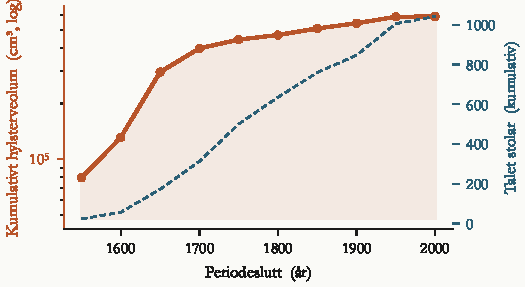
\includegraphics[width=\columnwidth]{figures/fig-expansion-en.pdf}
\caption{Cumulative morphospace expansion. Rust line: convex hull volume (log scale). Teal dashed: cumulative chair count. Each successive 50-year period contributes genuinely novel form regions.}
\label{fig:expansion}
\end{figure}

\textbf{The landscape shifts significantly between periods} (Proposition 4). The mean Wasserstein-1 distance between consecutive 50-year periods is 14.4~cm (H), 8.2~cm (W), and 5.9~cm (D). None of the ten period transitions show near-zero distance. The landscape is dynamic.

Figure~\ref{fig:materialstream} shows the material composition of the corpus over time. The successive waves; from oak through walnut, mahogany, steel, and plastic; visualize the material streams that drive landscape change (Proposition 4). Figure~\ref{fig:latency} demonstrates the latency hypothesis (Proposition 2): when a new material enters the corpus, its centroid initially clusters near the existing morphospace center; geometric divergence follows only after the material-specific operations are discovered and exploited.

\begin{figure}[!t]
\centering
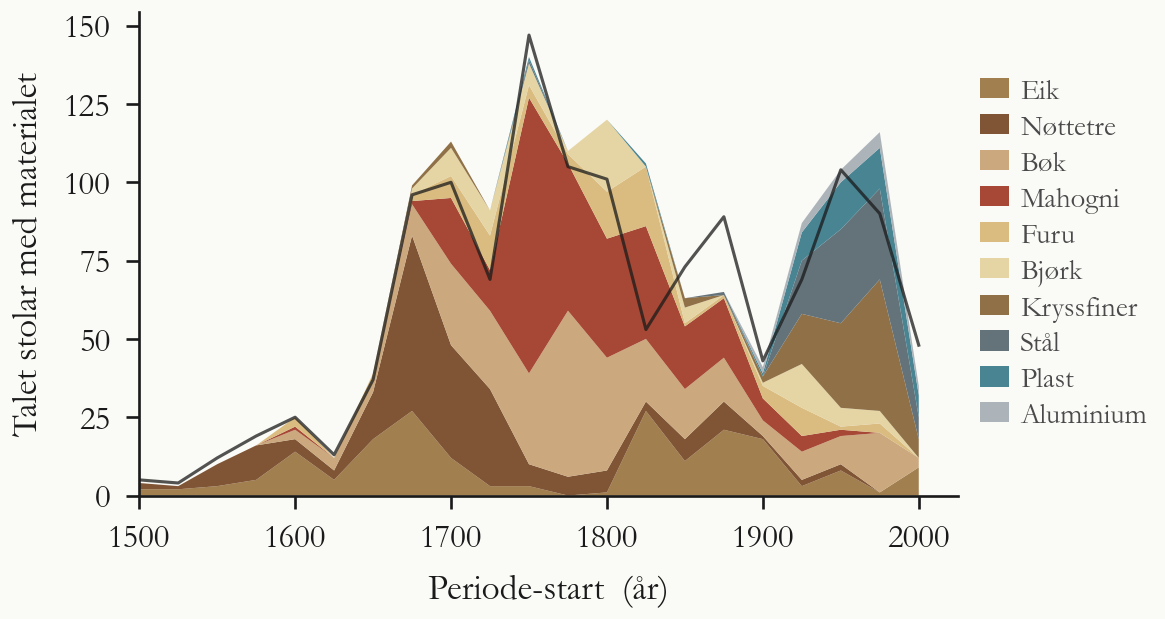
\includegraphics[width=\columnwidth]{figures/fig-materialstream-en.png}
\caption{Material streams across 500 years. Each stratum shows the count of chairs per 50-year period by primary material. Successive waves (oak, walnut, mahogany, steel, plastic) drive cumulative morphospace expansion.}
\label{fig:materialstream}
\end{figure}

\begin{figure}[!t]
\centering
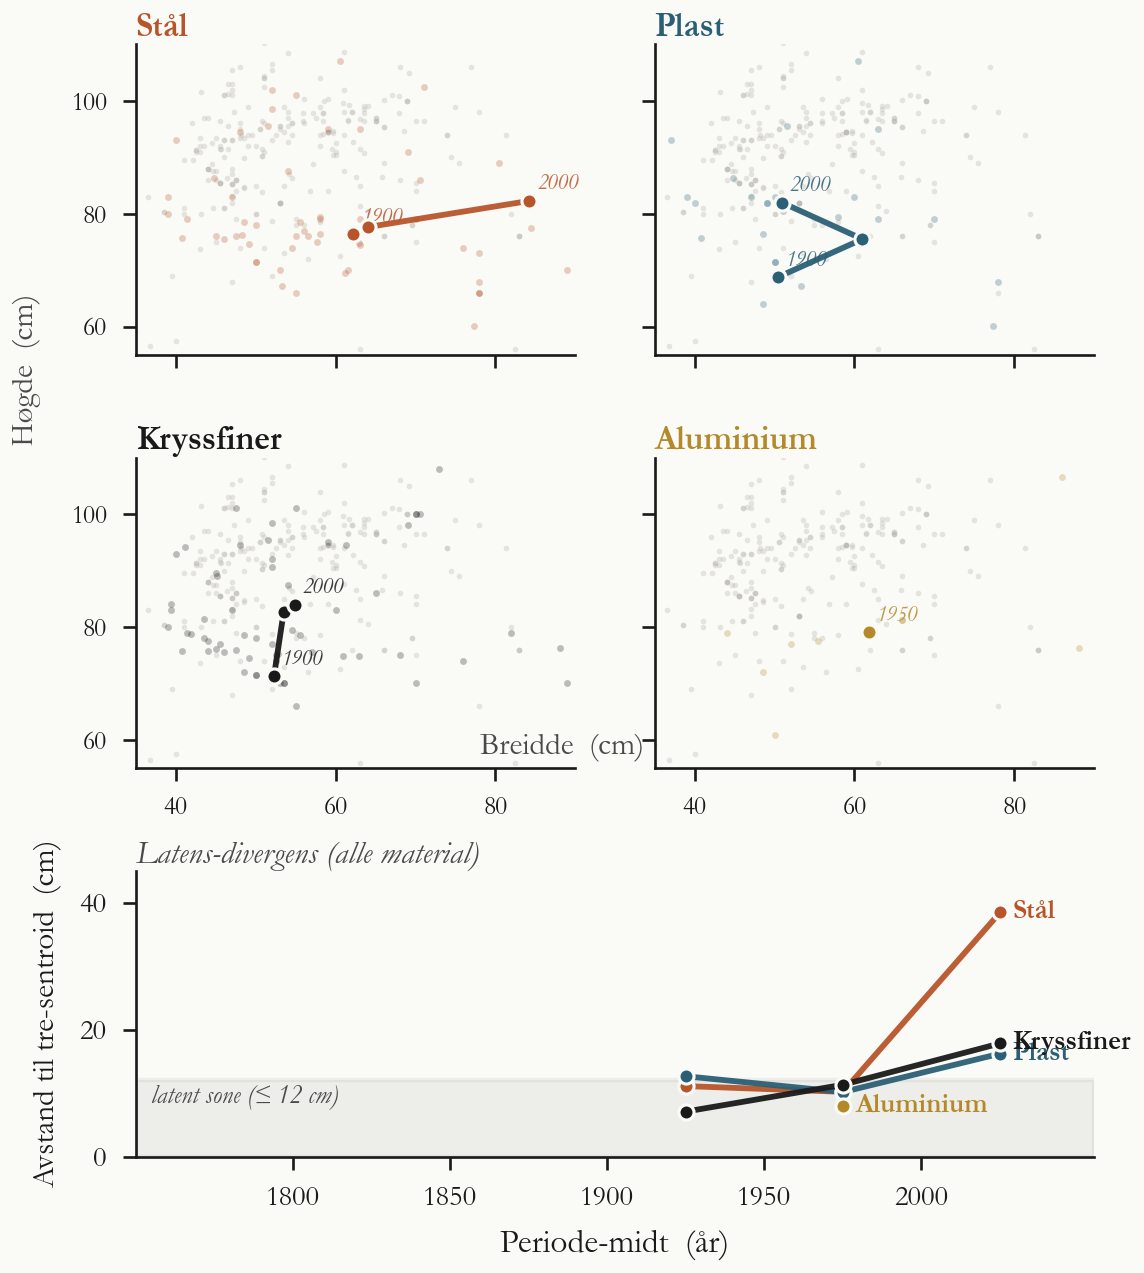
\includegraphics[width=\columnwidth]{figures/fig-materiallatency-en.png}
\caption{Material latency. Top panels: morphospace centroids for four materials (steel, plastic, plywood, aluminum) plotted against the full corpus (gray). Arrows trace centroid movement over time. Bottom panel: latency-divergence timeline showing that geometric divergence follows material introduction with a systematic lag.}
\label{fig:latency}
\end{figure}

\subsection{Robustness and falsification}

All 84 test-subset combinations (6 tests $\times$ 14 subsets) produce results consistent with the full-corpus findings. These are not 84 independent tests; the subsets overlap substantially. However, the consistency across deliberately adversarial hold-outs (museum shift, century removal, style removal) provides evidence that the findings are not artifacts of a single collection, period, or style category.

Seven direct falsification tests target the theory's postulates: non-confounding of predictors (Proposition 2), non-zero landscape shifts (Proposition 4), and non-uniform non-random-walk distributions (Proposition 5). All seven hold with $p$-values below $10^{-63}$ for the strongest tests.

No postulate is falsified in the dataset. Four additional tests were attempted and dropped for insufficient effect size (OU mean reversion, multi-agent MI uplift, substrate-independence excess, CV collapse during style dominance); these are documented transparently as negative or inconclusive results. The theory is not confirmed by cherry-picking; it survives systematic testing with pre-registered metrics.
